\begin{figure*}
    \begin{subfigure}[h]{0.45\textwidth}
        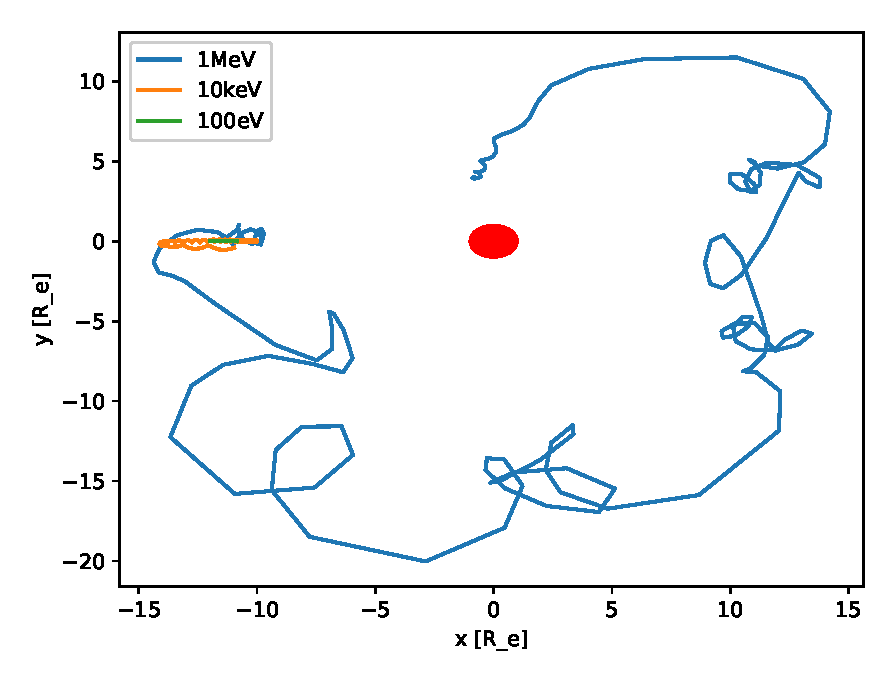
\includegraphics[width=\textwidth]{Figures/Trajectories/trajectories-xy-43.eps}
        \caption{$x_0 = [-12.0,0.0,-1.0]R_E$, $xy$-plane.}
        \label{fig:traj-a}
    \end{subfigure}
    \hfill
    \begin{subfigure}[h]{0.45\textwidth}
        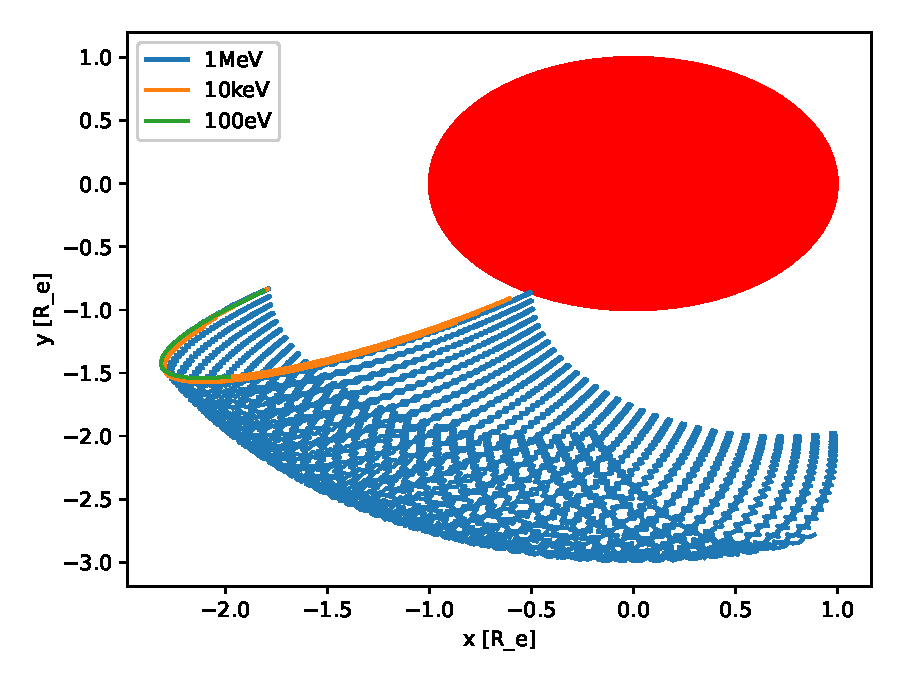
\includegraphics[width=\textwidth]{Figures/Trajectories/trajectories-xy-11.eps}
        \caption{$x_0 = [-2.0,-1.0,0.0]R_E$, $xy$-plane.}
        \label{fig:traj-b}
    \end{subfigure}
    \vfill
    \begin{subfigure}[h]{0.45\textwidth}
        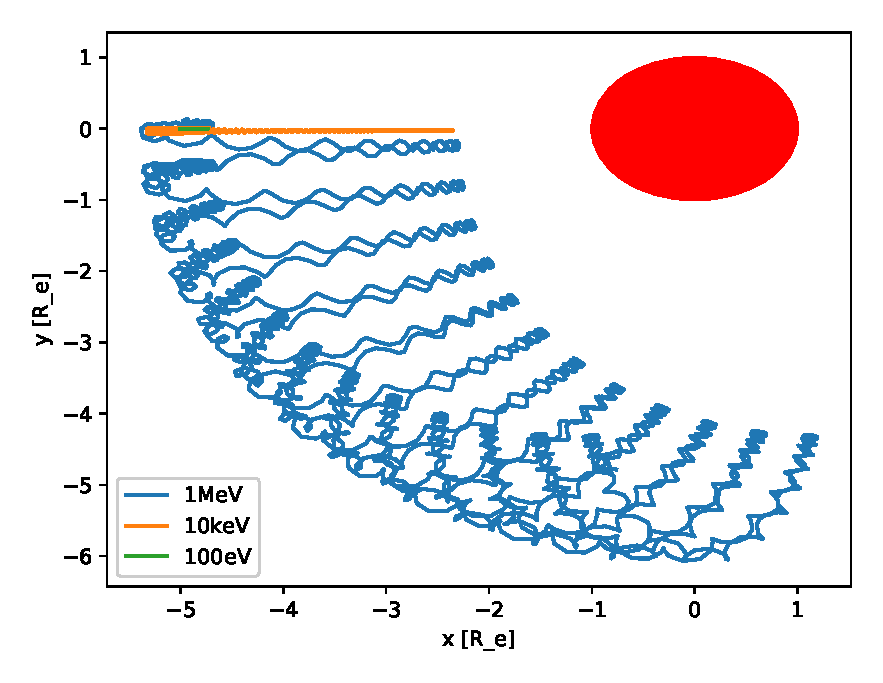
\includegraphics[width=\textwidth]{Figures/Trajectories/trajectories-xy-36.eps}
        \caption{$x_0 = [-5.0,0.0,-1.0]R_E$, $xy$-plane.}
        \label{fig:traj-c}
    \end{subfigure}
    \hfill
    \begin{subfigure}[h]{0.45\textwidth}
        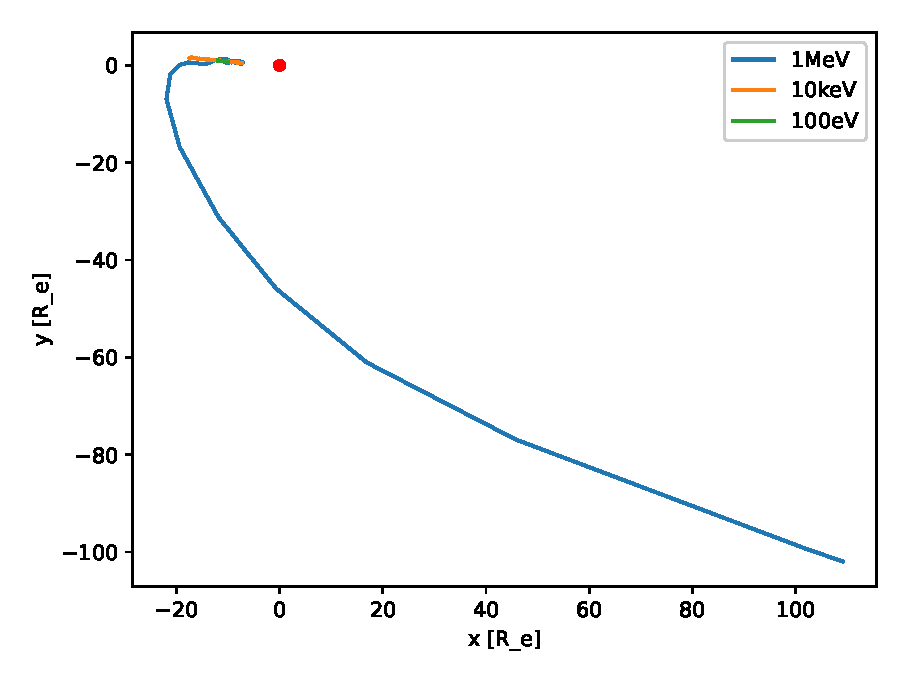
\includegraphics[width=\textwidth]{Figures/Trajectories/trajectories-xy-98.eps}
        \caption{$x_0 = [-12.0,1.0,1.0]R_E$, $xy$-plane.}
        \label{fig:traj-d}
    \end{subfigure}
    \vfill
    \begin{subfigure}[h]{0.45\textwidth}
        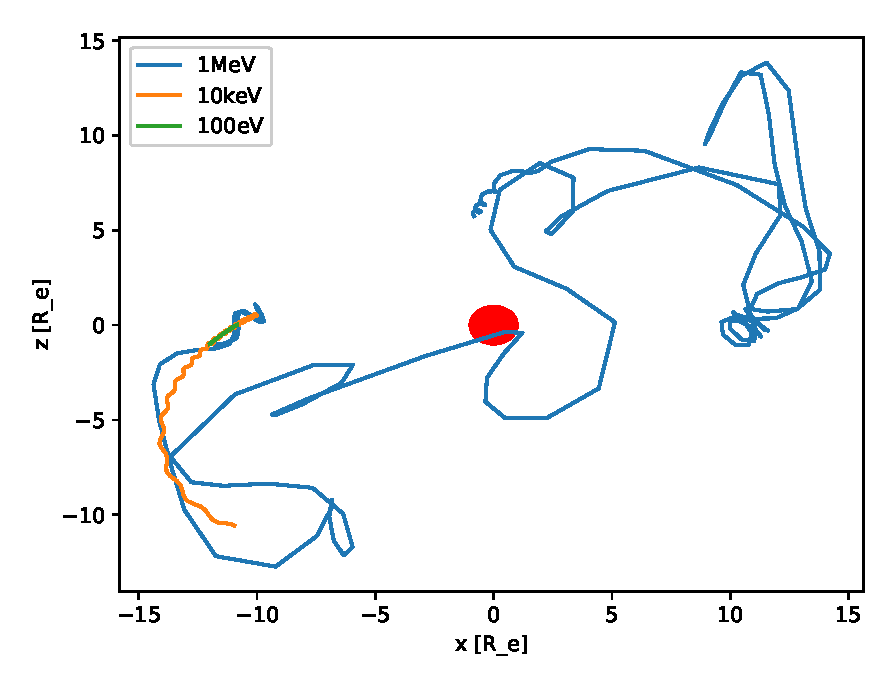
\includegraphics[width=\textwidth]{Figures/Trajectories/trajectories-xz-43.eps}
        \caption{$x_0 = [-12.0,0.0,-1.0]R_E$, $xz$-plane.}
        \label{fig:traj-e}
    \end{subfigure}
    \hfill
    \begin{subfigure}[h]{0.45\textwidth}
        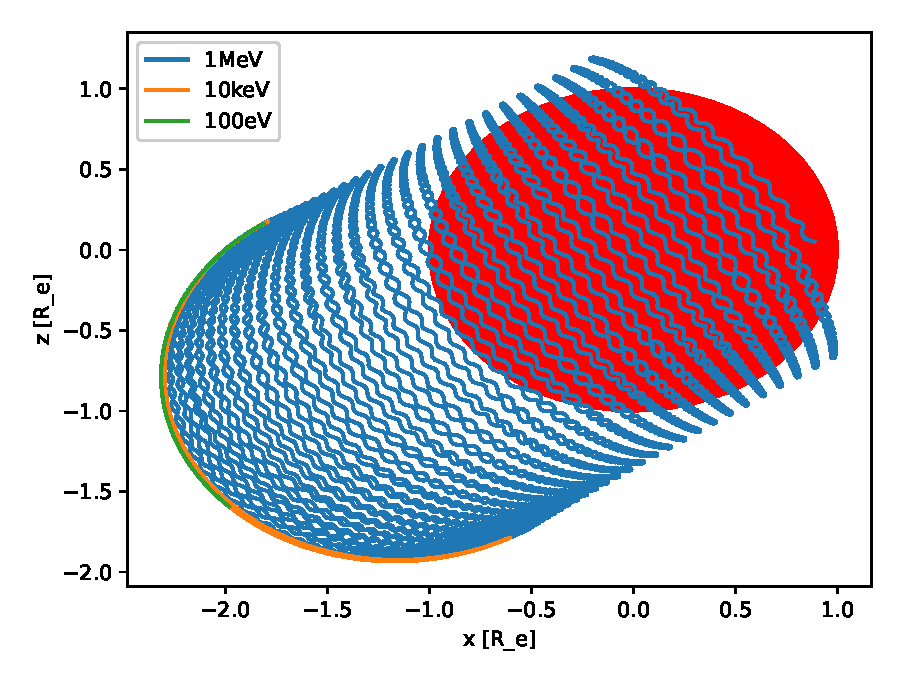
\includegraphics[width=\textwidth]{Figures/Trajectories/trajectories-xz-11.eps}
        \caption{$x_0 = [-2.0,-1.0,0.0]R_E$, $xz$-plane.}
        \label{fig:traj-f}
    \end{subfigure}
    \vfill
    \begin{subfigure}[h]{0.45\textwidth}
        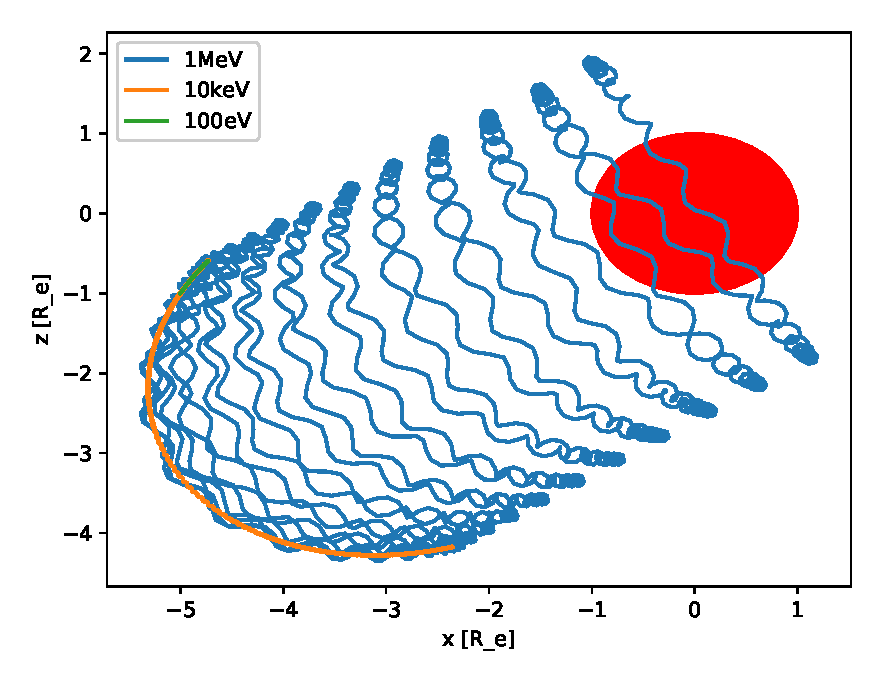
\includegraphics[width=\textwidth]{Figures/Trajectories/trajectories-xz-36.eps}
        \caption{$x_0 = [-5.0,0.0,-1.0]R_E$, $xz$-plane.}
        \label{fig:traj-g}
    \end{subfigure}
    \hfill
    \begin{subfigure}[h]{0.45\textwidth}
        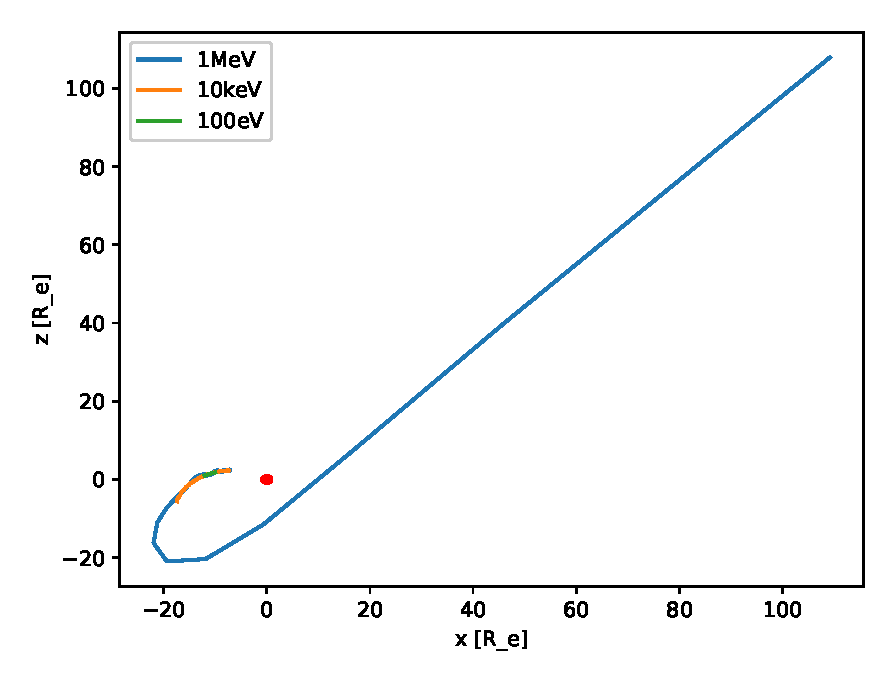
\includegraphics[width=\textwidth]{Figures/Trajectories/trajectories-xz-98.eps}
        \caption{$x_0 = [-12.0,1.0,1.0]R_E$, $xz$-plane.}
        \label{fig:traj-h}
    \end{subfigure}
    \caption{Trajectories of 100eV, 10keV and 1MeV protons projected onto the $xy$- and 
    $xz$-planes. The initial positions of the protons are noted in the subcaptions.}
    \label{fig:trajectories}
\end{figure*}